\chapter{\acrshort{ux} \& \acrshort{ui} design} \label{chapter4}

    The interface of an application represents the main component with which the user interacts directly. By offering a predictable, concise, and consistent design, students will be motivated to use our solution. Hence, we prioritize the appearance of our application and the ideas that might lead to an overall increased satisfaction level.

\section{Requirements} \label{4:requirements}

    Our application is conceived to be suitable for Android, iOS, and web users. Thus, we create a design that contains good graphics for any device used by students.
    
    According to a study \cite{flutter2020experience} performed in 2020 about developing applications in Flutter (the framework we use for implementation and which is further described in section \ref{chapter5}), this technology offers a high degree of flexibility in modeling an attractive design. Simultaneously, it offers a fast implementation process due to an extensive range of ready-to-use widgets\footnote{https://flutter.dev/docs/development/ui/widgets}, which can also be adapted depending on the device used, having a single codebase.
    
    The \acrshort{ui} elements we use in this application are \textit{Material Design}\footnote{https://materialdesignicons.com/} and \textit{Font Awesome}\footnote{https://fontawesome.com/} icons in an outlined variant and \textit{unDraw}\footnote{https://undraw.co/} illustrations. These provide a modern and catchy look to our solution so that students are encouraged to use it.
    
    Moreover, to ensure suitable formatting of our pages for different screen sizes, we position the graphic elements relative to each other to preserve the proportions.

\section{Feedback questionnaire} \label{4:feedback_questionnaire}

    \subsection{Motivation} \label{4:motivation}

    To collect adequate opinions from students regarding their classes, we carefully chose the set of questions, further described in section \ref{4:chosen_questions}. These are as varied as possible and cover a wide range of possible aspects that can be improved, such as lectures, applications, or homework.
    
    Considering that constructive feedback is always based on sincere thoughts and individual student voices, it is crucial to collect as many free answers as possible through explicit wordings. The thinking of students should not be limited only to the selection of some already predefined statements.
    
    However, time spent on a questionnaire determines whether to participate in completing it or not \cite{roszkowski1990}. Thus, single or multiple-choice queries, \textit{Likert} scale, and dropdowns questions should not be completely absent. These types allow students who do not want to compose much or describe their feelings to offer any echo, helpful in obtaining a certain kind of perceptible data \cite{reja2003questions}.
    
    Additionally, a well-composed form should not mark all fields as mandatory to be answered because some people may feel compelled to express their attitude even if they desire to abstain. Nevertheless, this freedom does not have to be complete either because some may be encouraged to quickly overlook and forget to have their say on the required topics. Furthermore, the more concrete a question is, the more an answer might contribute to class enhancement. A balanced combination of all these concepts can significantly influence how students perceive providing feedback in the educational domain.
    
	Students should be instructed on the role and purpose of this feedback form, more precisely why their opinions are meaningful, and explain how these influence the development of the educational process. Therefore, the probability of students completing this evaluation might increase if they will be informed that teachers seriously consider changes based on their observations.
	
	Although some believe that feedback is not entirely anonymous, it must be rigorously explained how all the data provided is stored in the database and that there is no connection between the name of a person and his answers. However, a reference must be maintained to specify whether a student has submitted the feedback form for a specific class as not to allow multiple times completion. Besides this, it must be stated that their viewpoints will never be forgotten and unused by simply publishing them on a statistics page, to be analyzed by future generations as well.
	
	\subsection{Structure} \label{4:structure}
	
	Before we composed the most appropriate questions, we organized them in several categories so that the mind of the person fulfilling is neither puzzled nor passed from one section to another one. Like the online course platform Moodle, the underlying divisions of the educational process include general accommodation questions, followed by a more profound investigation about the lecture, laboratory, seminar and applications, homework, percentage of participation in the overall class activities, and personal questions.
	
	Unlike Moodle, which focuses on feedback before taking the exam session, this application wants to collect reviews, including final evaluation impressions. Through this, future generation students can learn valuable insights, such as how difficult it is to understand the overall class theory or how hard it is to pass the exam. Therefore, in contrast to the Moodle direction, the purpose of the feedback form in this application is to aid teachers and students.
	
	Undoubtedly, by considering this approach, there is always a risk that specific students may suddenly change their thoughts about a class, which they may even have beloved, if the final examination does not go as well as they would have imagined or if it did not meet their expectations. Despite this fact, it must be considered that it will include the good, the bad, and the ugly whenever we open ourselves up to feedback. No matter how heavily someone might try, there is a remarkably tiny probability that negative comments and insults will be everlastingly null. Instead, the solution to which we must pay exclusive emphasis is based on identifying means that can substantially reduce criticism until we reach the ideal situation.
	
	Therefore, no student should ever address offensive words or false opinions, which do not respect the objective reality. Naturally, it is impossible to please everyone repeatedly. As a result, when those critiques show up, their reason must be identified and subsequently reflected on how their reappearance could be avoided.
	
	After establishing the categories, the manner of defining a question should not be neglected. The way an inquiry is asked may or may not encourage the receipt of a particular type of answer. For instance, by introducing a question like "\textit{What did you dislike about this class?}", we open ourselves for harsh responses like, "\textit{I did not like anything. I cannot stand this class.}". Nevertheless, if we are careful to immediately insert a follow-up question like "\textit{What do you suggest to improve the negative aspects mentioned before?}", the presumption of receiving a pragmatic justification is not guaranteed but increases noticeably. Therefore, the most powerful tool that guides someone in this context is represented by anticipating possible comments and thinking on how to induce the interviewees to envisage by providing their most valuable feedback.
	
	\subsection{Chosen questions} \label{4:chosen_questions}
	
    Among the questions \cite{questionestablishment} we added in this application are:
    
    \begin{itemize}
            \setlength{\topsep}{0.5pt}
            \setlength{\itemsep}{0.5pt}
            \setlength{\parsep}{0.5pt}
            \item \textbf{"\textit{How does this class contribute to your stress level?}"}: as it is well known, no one desires to study or carry out their activities in a tense environment. Stressful experiences contribute to a significant impact on the mood of students, being at the same time a critical factor that could cause them to express their anger in a feedback form. This indignation might obscure positive thoughts of students about a class, opinions that could have even acknowledged that the theory learned throughout the semester is helpful to them in their future careers. As a result, teachers should permanently challenge students to reach their maximum potential while maintaining certain limits. Of course, students need to be pushed out of their comfort zone but taking care to have at the same time a balanced ambiance.

            \item \textbf{"\textit{Identify your effort level for this class.}"}: this is a handy question for both students and teachers, thus making them aware of how far a class is located compared to other disciplines that offer the same number of credits in terms of difficulty.
            
            \item \textbf{"\textit{What is one aspect you would change about this class? How do you think it should be revised?}"}: by aggregating the answers to this question, generations of students to come will be aware of the existing imperfections from a specific class and will be able to propose multiple possibilities for improvement. 
            
            \item \textbf{"\textit{What advice would you give to future generations of students about this class?}"}: playing a prominent role in maintaining the connection between students, this question contributes to the accountability of older students while the youngest benefit from various opinions.
            
            \item \textbf{"\textit{What are you proud of accomplishing in this class?}"}: it is genuinely essential to highlight accomplished successes to arouse the interest and motivation of students to learn and manage to achieve results at least as satisfying as their previous generation. Therefore, this question stimulates continuous progress and encourages educational advancement. Students will be boosted to get out of their comfort zone and set their sights as high as possible. Without any quest to look forward to, there is always a real threat of not valuing our capabilities enough.
            
            \item \textbf{"\textit{Did you take the exam?}"}: unlike other queries that can receive more complex answers, this is a straightforward inquiry to identify the pass rate of a specific class, one of the most sought-after information among students.
            
            \item \textbf{"\textit{How much time did you have to prepare for the exam?}"}: one of the questions that students frequently ask to help them manage their schedule better and realize how dense the information to be retained is.
            
            \item \textbf{"\textit{What grade did you get in this class?}"}: short and to the point question, which helps students easily visualize their level compared to others or, for those who are going to study the discipline, the overall average grade.
            
            \item \textbf{"\textit{Do you think the knowledge gained will be useful in your future career?}"}: naturally, not all the theories studied will always be advantageous in our professional development. Everyone has their passions, being more or less attracted to specific topics. However, the purpose of this question is to identify cases in which a student is particularly attracted to a subject. Results obtained in this category can be subsequently interpreted by both students and teachers, thus serving in the continuous process of remodeling the discipline.
            
            \item \textbf{"\textit{Was the exam easier than in other classes that offer the same number of credits?}"}: a question that offers an insight about the comparison between different classes and whether there is a level of balance or not. 
            
    \end{itemize}

\section{Prototyping} \label{4:prototyping}

    \subsection{Initial design} \label{4:initial_design}
    
    Based on our experience, we confirm that the appearance of an application influences users on whether to continue using it or not. As a result, we pay great attention to creating a concise, attractive, and easy-to-understand interface. Along with these characteristics, we consider the idea of having a uniform, airy, and user-friendly layout.
    
    According to a study conducted in 2009 \cite{2009design}, conceiving the right design for mobile devices is a challenging process. As we strive to ensure an excellent level of satisfaction to students, the action of defining a good-looking prototype preceded the process of implementing the architecture itself, described in chapter \ref{chapter5}.
    
    We sketched the aspect of our project in Figma\footnote{https://www.figma.com/}, taking care to maintain the theme of the already implemented modules (fig. \ref{4:fig:figma_prerequisites} - \ref{4:fig:figma_statistics}).
    
    \begin{figure}[!ht]
        \centering
        \begin{minipage}[b]{0.32\textwidth}
            \captionsetup{justification=centering}
            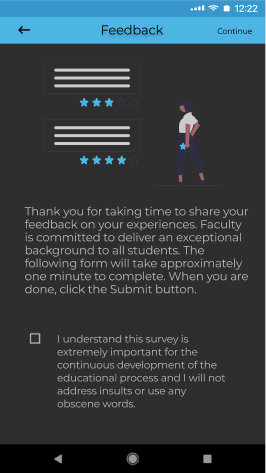
\includegraphics[width=\textwidth]{figures/app/initial/prerequisites.png}
            \caption{Feedback prerequisites mock-up}
            \label{4:fig:figma_prerequisites}
        \end{minipage}
        \hfill
        \begin{minipage}[b]{0.318\textwidth}
            \captionsetup{justification=centering}
            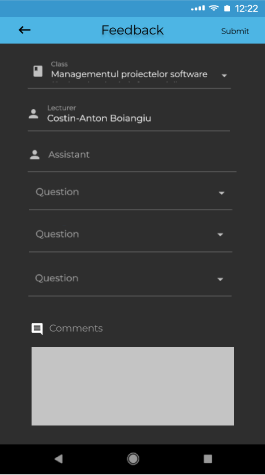
\includegraphics[width=\textwidth]{figures/app/initial/form.png}
            \caption{Feedback questionnaire mock-up}
            \label{4:fig:figma_form}
        \end{minipage}
        \hfill
        \begin{minipage}[b]{0.321\textwidth}
            \captionsetup{justification=centering}
            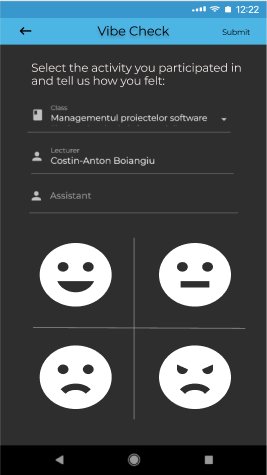
\includegraphics[width=\textwidth]{figures/app/initial/vibe_check.png}
            \caption{Vibe check mock-up}
            \label{4:fig:figma_vibe_check}
        \end{minipage}
    \end{figure}
    
    \begin{figure}[!ht]
        \centering
        \begin{minipage}[t]{0.32\textwidth}
            \captionsetup{justification=centering}
            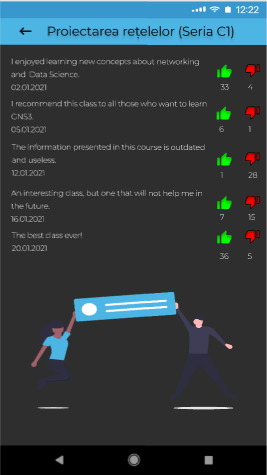
\includegraphics[width=\textwidth]{figures/app/initial/opinions.png}
            \caption{Opinions page mock-up}
            \label{4:fig:figma_opinions}
        \end{minipage}
        \hfill
        \begin{minipage}[t]{0.663\textwidth}
            \captionsetup{justification=centering}
            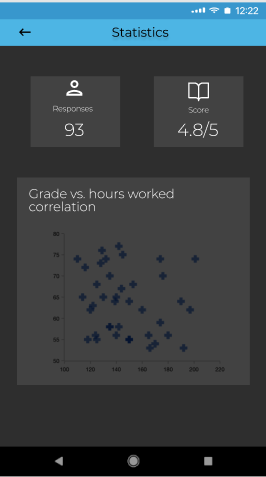
\includegraphics[width=0.48\textwidth]{figures/app/initial/statistics_1.png}
            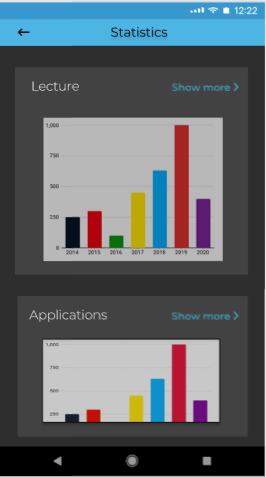
\includegraphics[width=0.48\textwidth]{figures/app/initial/statistics_2.png}
            \caption{Statistics overview mock-up}
            \label{4:fig:figma_statistics}
        \end{minipage}
    \end{figure}
    
    Initially, the role of the prerequisites page (fig. \ref{4:fig:figma_prerequisites}) was thought to inform students about the approximate time required to complete a feedback questionnaire and agree to provide constructive information. However, we decided to reduce the number of clicks a user must perform and removed this page.
    
    \begin{wrapfigure}{r}{0.35\columnwidth}
            \centering
            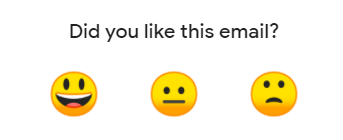
\includegraphics[width=0.42\columnwidth]{figures/google_emoticons.png}
            \captionsetup{labelsep=space, textformat=empty}
            \caption{Emoticons used by Google Maps Timeline email template}
            \label{4:fig:google_emoticons}
    \end{wrapfigure}
    
    Moreover, apart from the classic form students need to complete at the end of each academic semester, we sketched a \textit{vibe check} feature. Its role is to collect information about the mood of students after attending a course, laboratory, or seminar. The interface presented is intuitive and uses emoticons to collect data from students. This idea was inspired by the template used by Google Maps\footnote{https://www.google.com/maps} Timeline emails to collect impressions from students, as illustrated in figure \ref{4:fig:google_emoticons}.
    
    \subsection{Final design} \label{4:final_design}
    
    We followed an iterative process of design development to reach a pleasant and intuitive interface for our application. Overall, we maintained the ideas outlined in the previous section \ref{4:initial_design}, to which we added minor improvements.
    
    To ensure that our application benefits from a clean and catchy layout with smooth transition between pages and readable information, we constantly received advice from a \acrshort{ux} \& \acrshort{ui} designer.
    
    In terms of \acrshort{ux}, the feedback questionnaire (fig. \ref{4:fig:feedback_form_page}) was initially accessible only from a class page by pressing a suggestive icon in the top right corner. Since students could easily omit this feature, we implemented a notification on the Home page that announces students how many feedback forms are still available to be completed (fig. \ref{4:fig:feedback_nudge}).
    
    By pressing the notification, users are redirected to a feedback checklist page (fig. \ref{4:fig:feedback_checklist}) that displays a list of all the forms that were already submitted or not, thus providing an overview of them. Naturally, students can navigate to
    
    \begin{figure}[!ht]
        \centering
        \begin{minipage}[t]{0.315\textwidth}
            \captionsetup{justification=centering}
            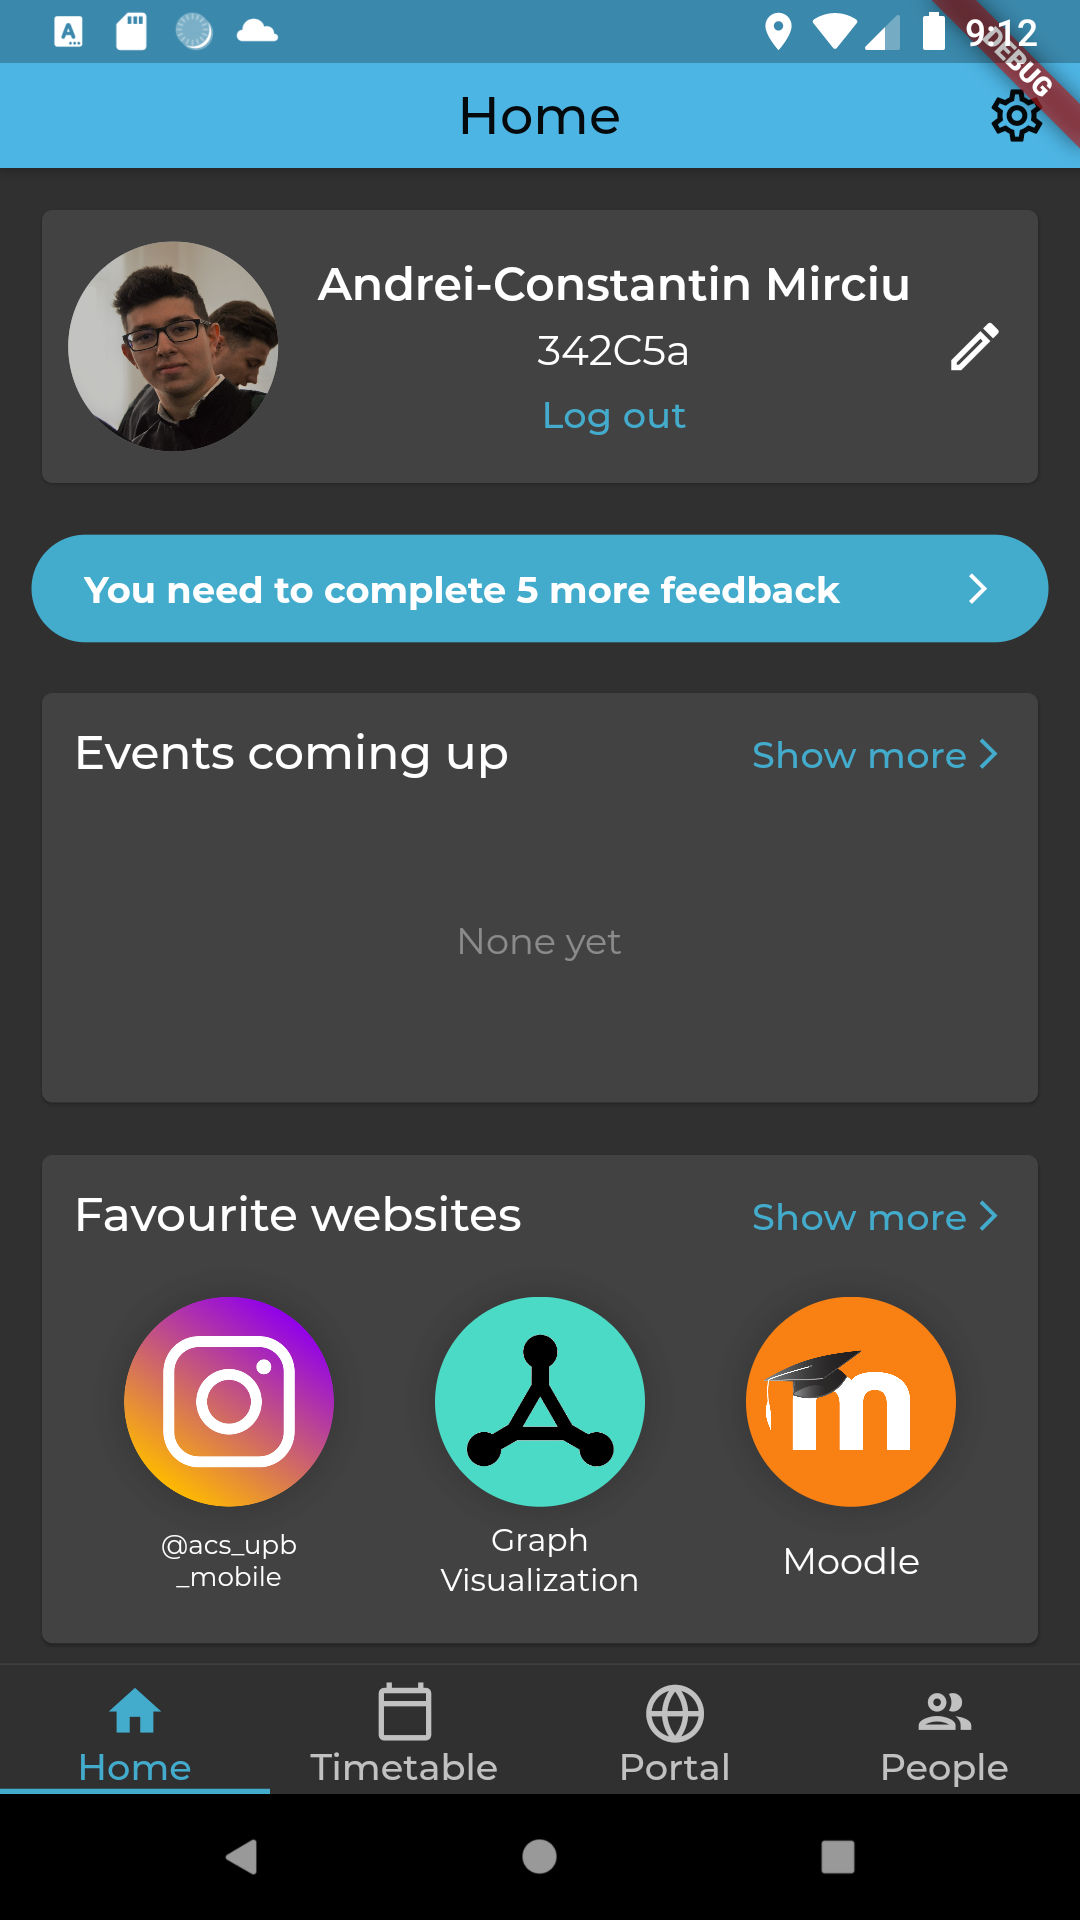
\includegraphics[width=\textwidth]{figures/app/final/feedback_nudge.png}
            \caption{Feedback notification on the Home page}
            \label{4:fig:feedback_nudge}
        \end{minipage}
        \hfill
        \begin{minipage}[t]{0.315\textwidth}
            \captionsetup{justification=centering}
            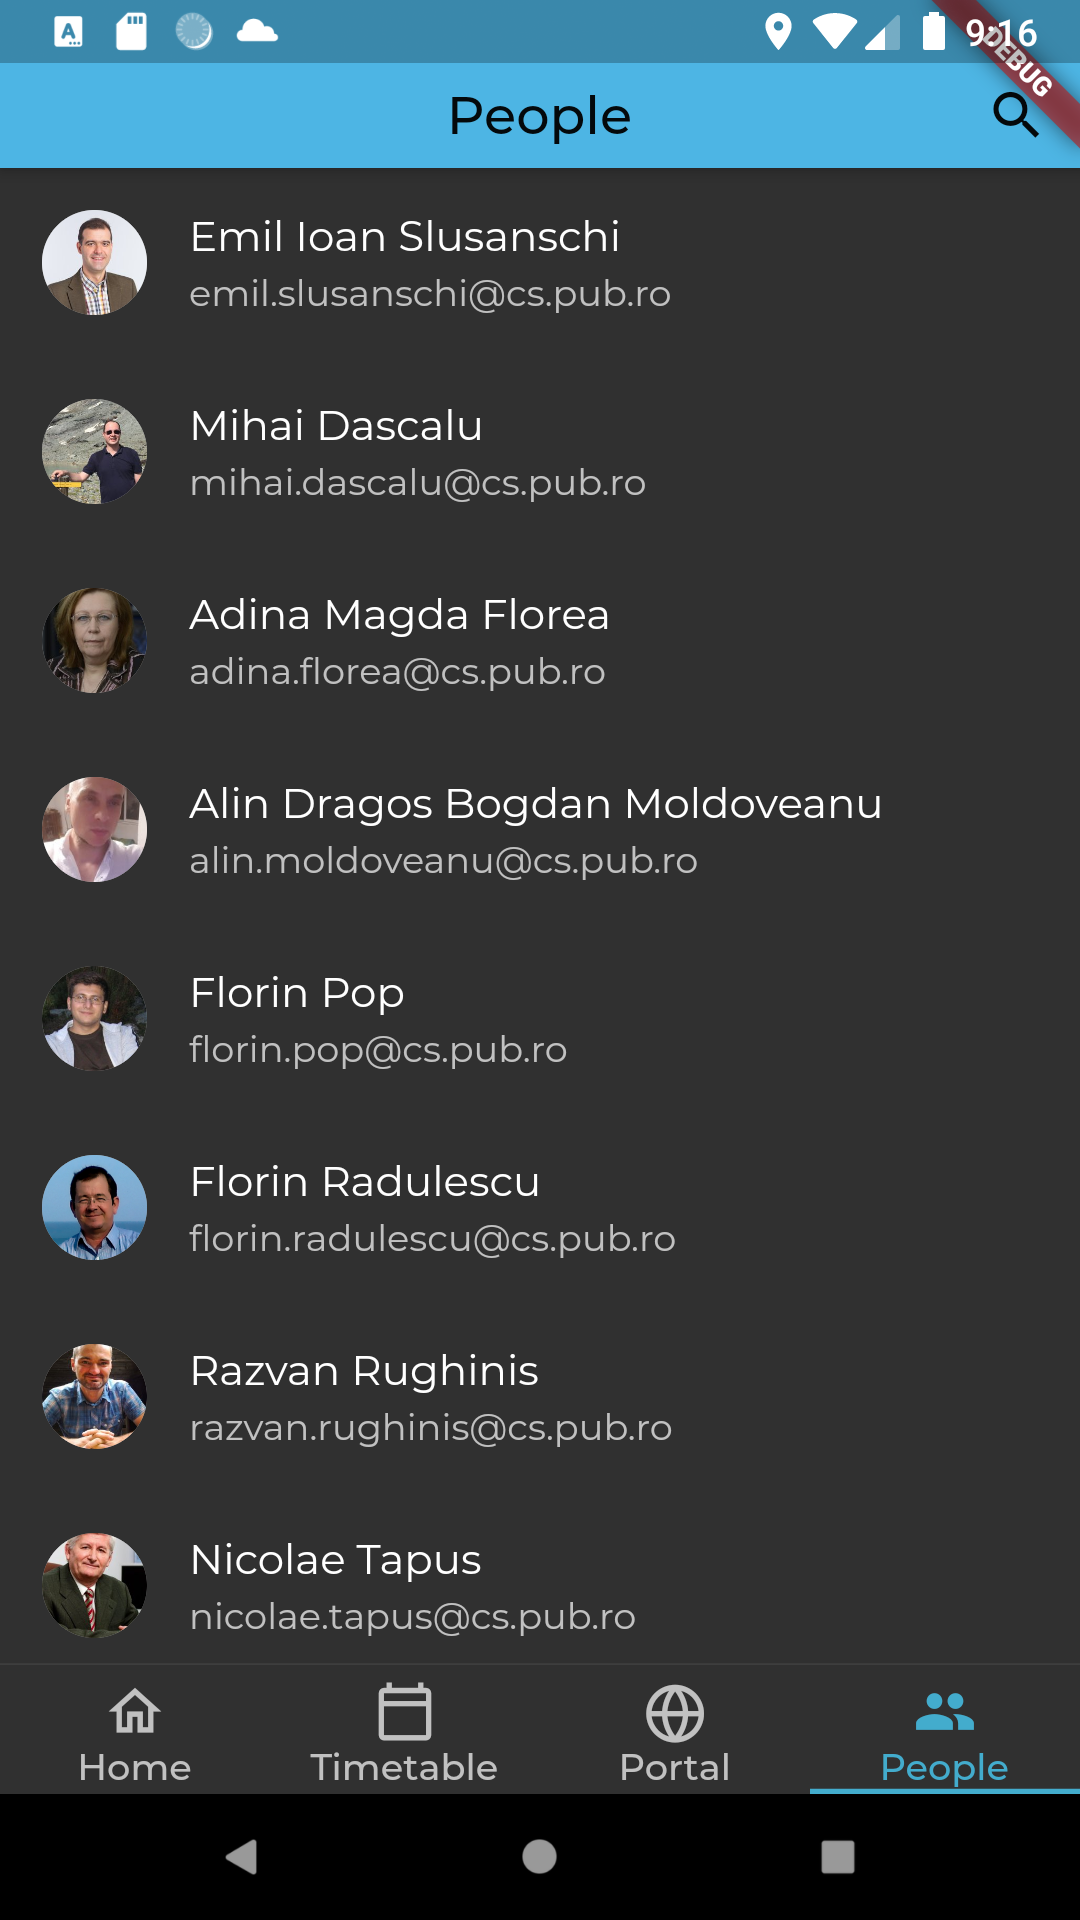
\includegraphics[width=\textwidth]{figures/app/final/people_page.png}
            \caption{People page}
            \label{4:fig:people_page}
        \end{minipage}
        \hfill
        \begin{minipage}[t]{0.315\textwidth}
            \captionsetup{justification=centering}
            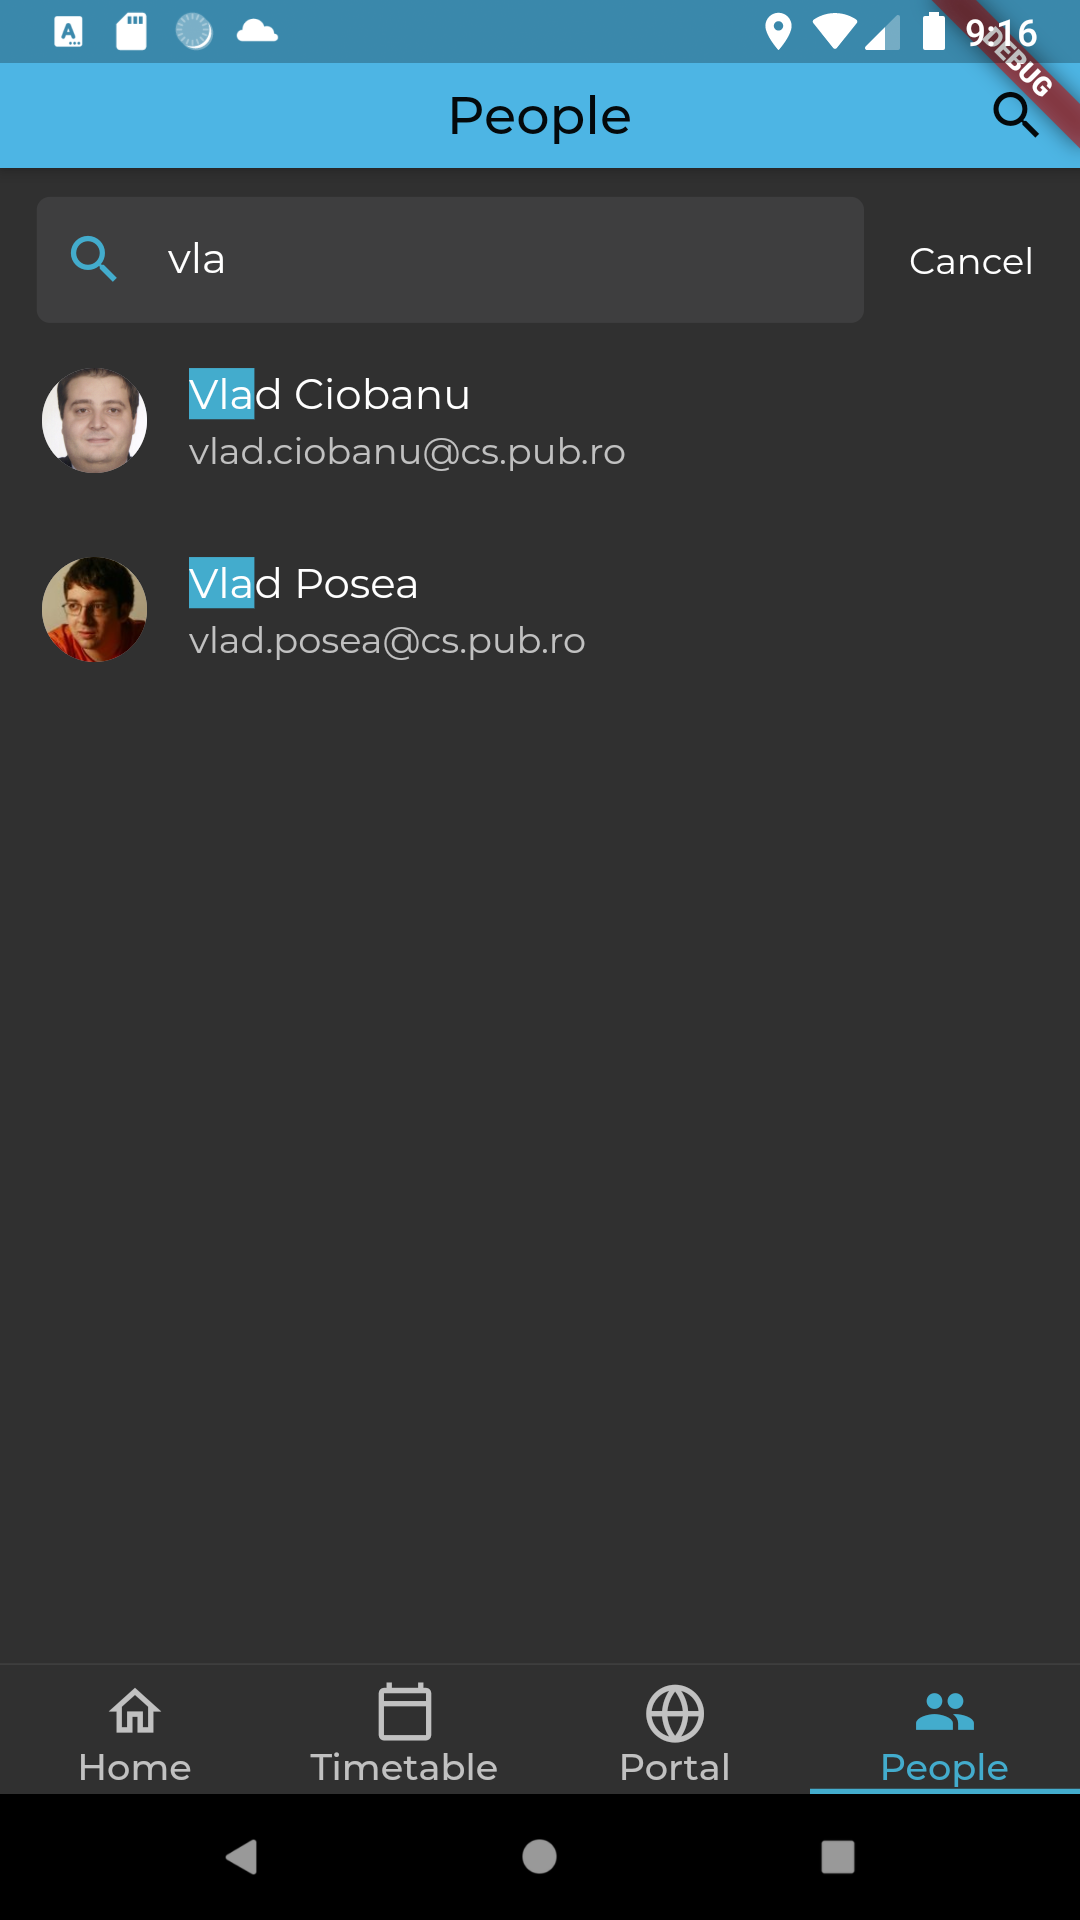
\includegraphics[width=\textwidth]{figures/app/final/people_search.png}
            \caption{People page search option}
            \label{4:fig:people_search}
        \end{minipage}
    \end{figure}

    \begin{figure}[!ht]
        \centering
        \begin{minipage}[t]{1.1\textwidth}
            \captionsetup{justification=centering}
            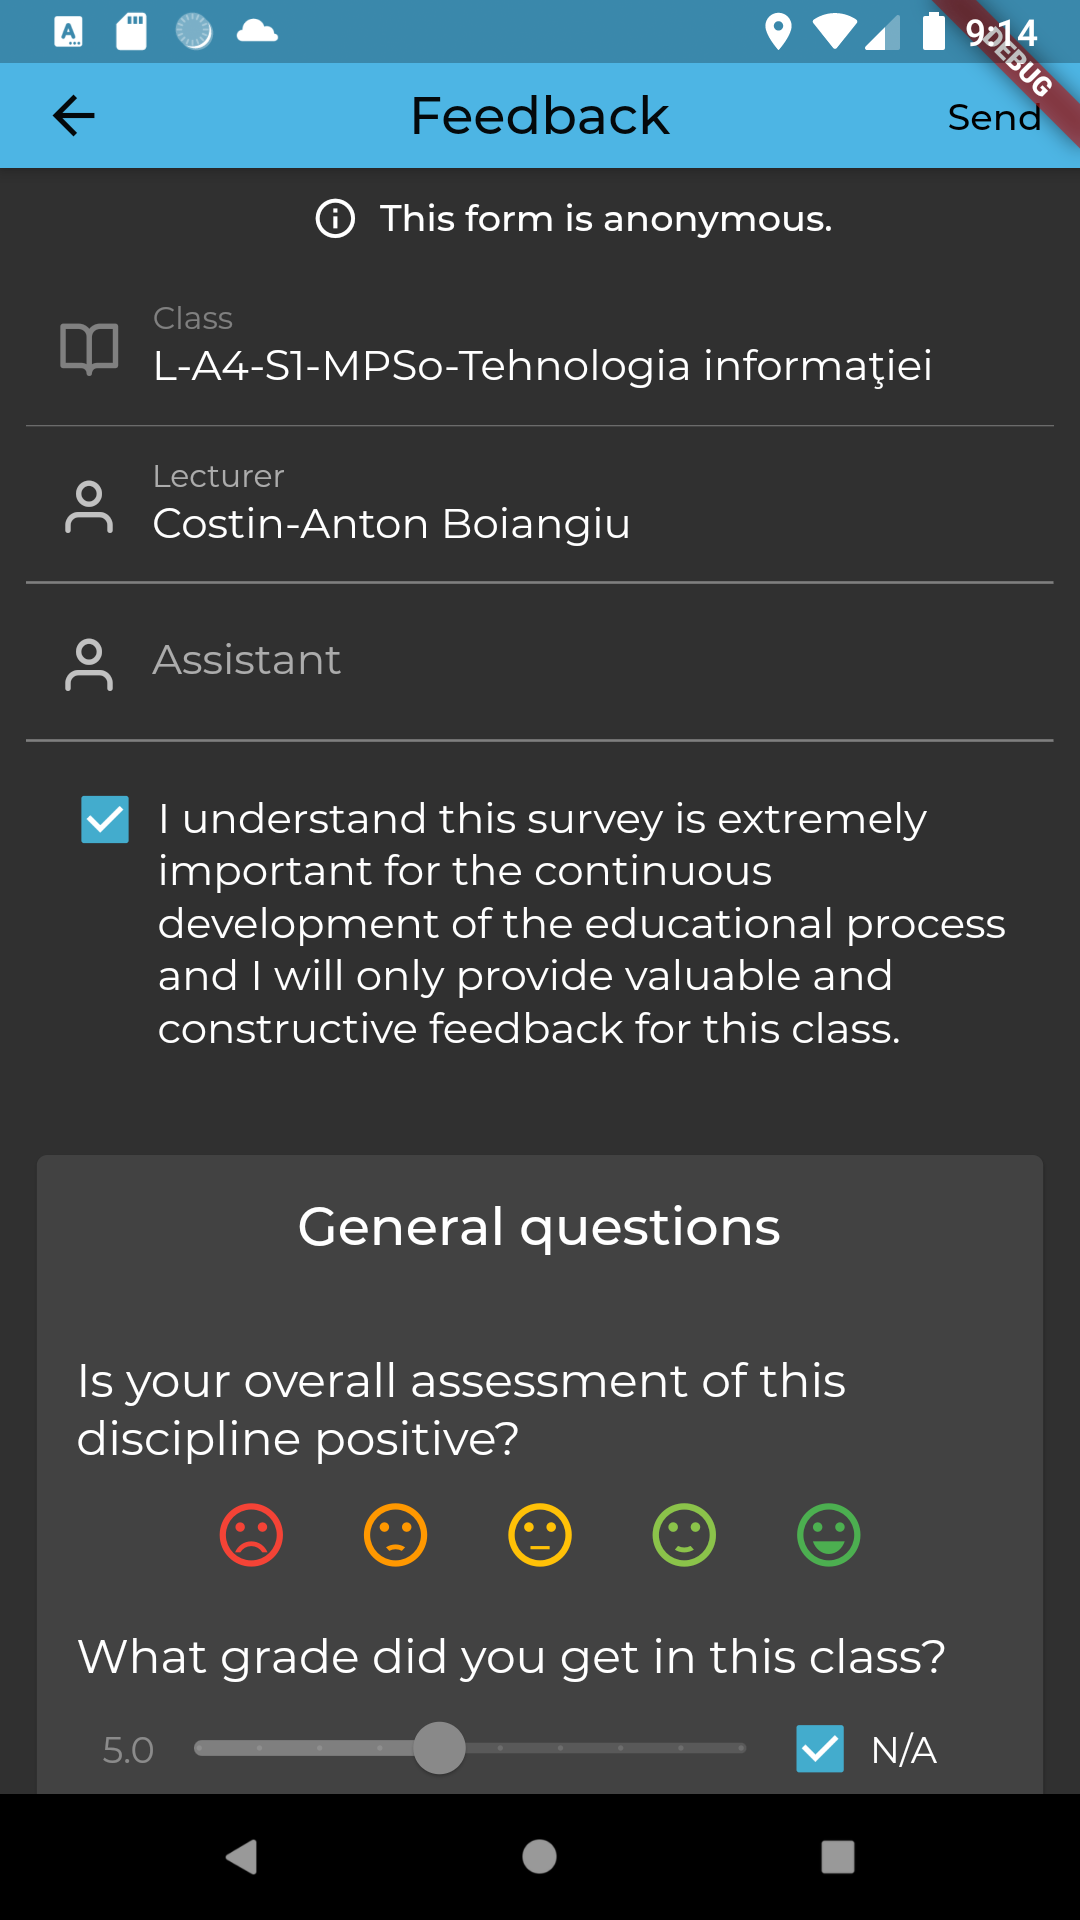
\includegraphics[width=0.3\textwidth]{figures/app/final/feedback_form_1.png}
            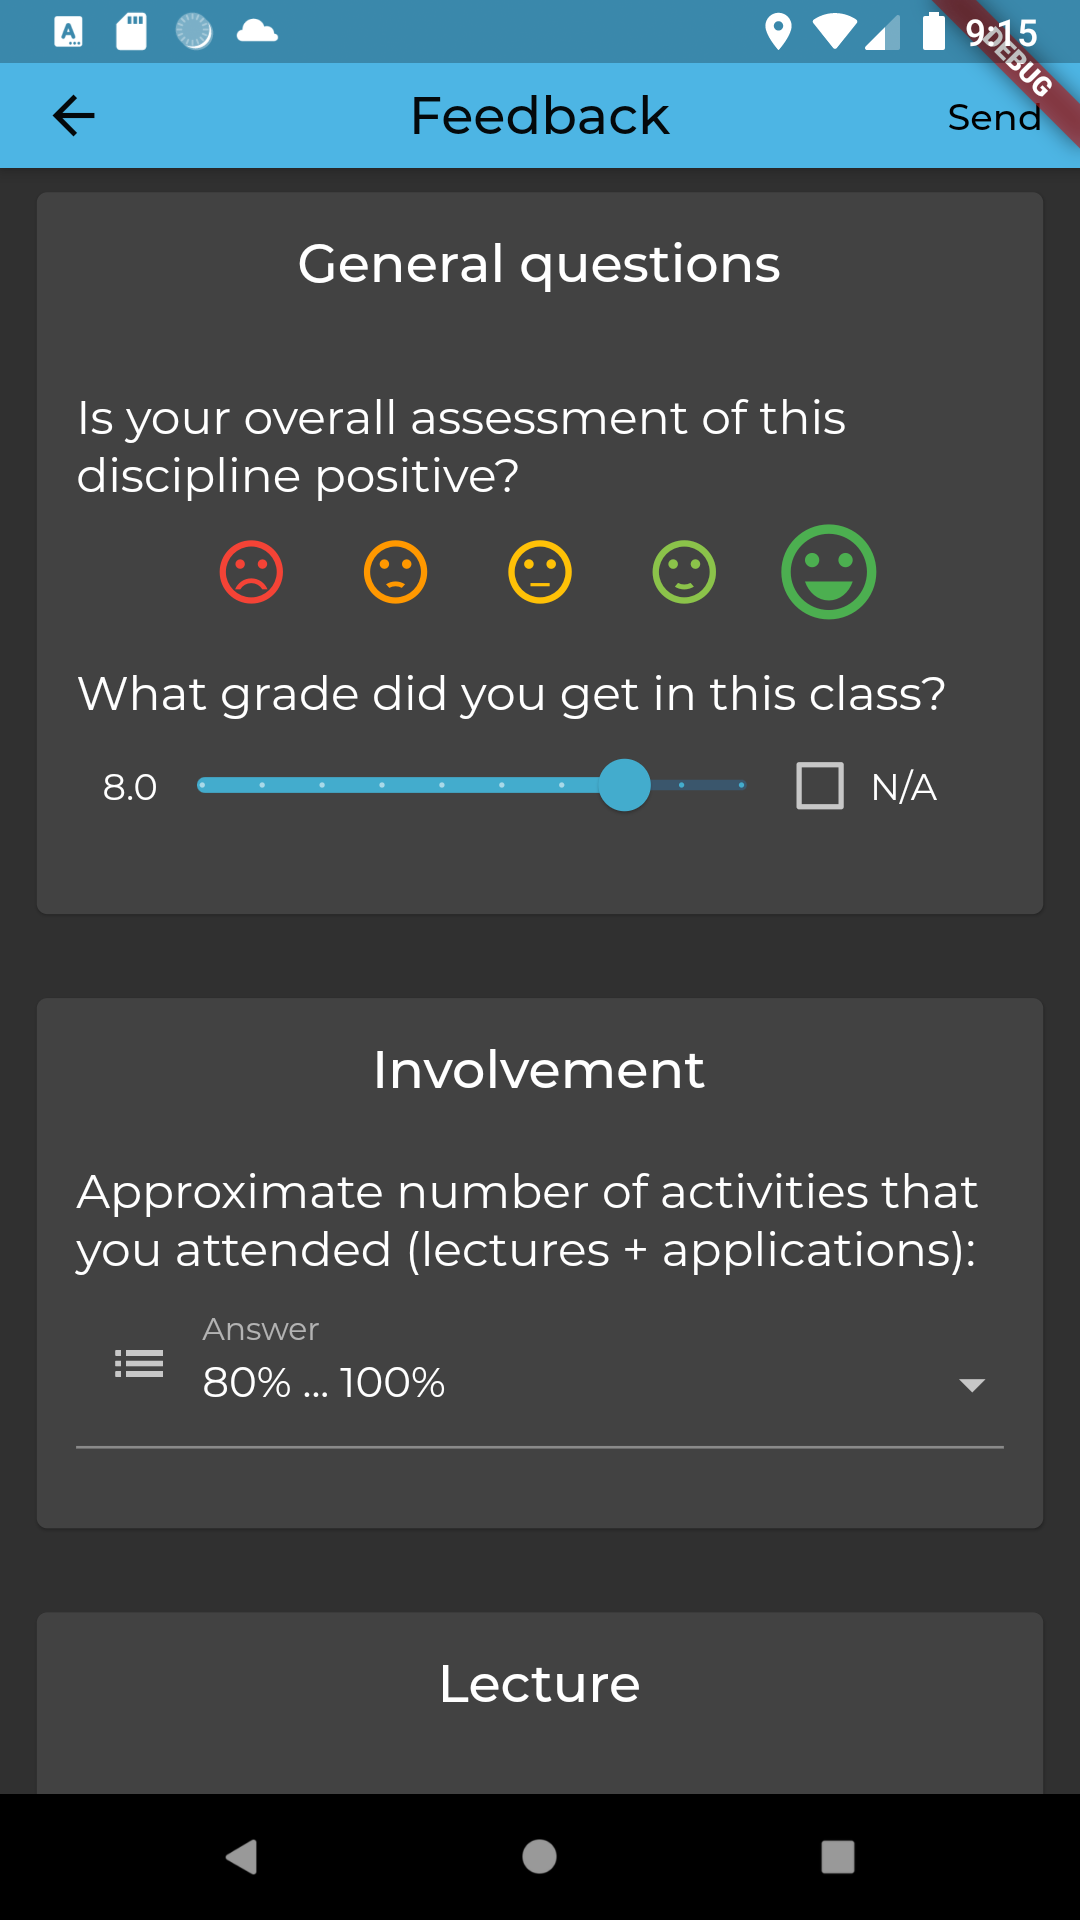
\includegraphics[width=0.3\textwidth]{figures/app/final/feedback_form_2.png}
            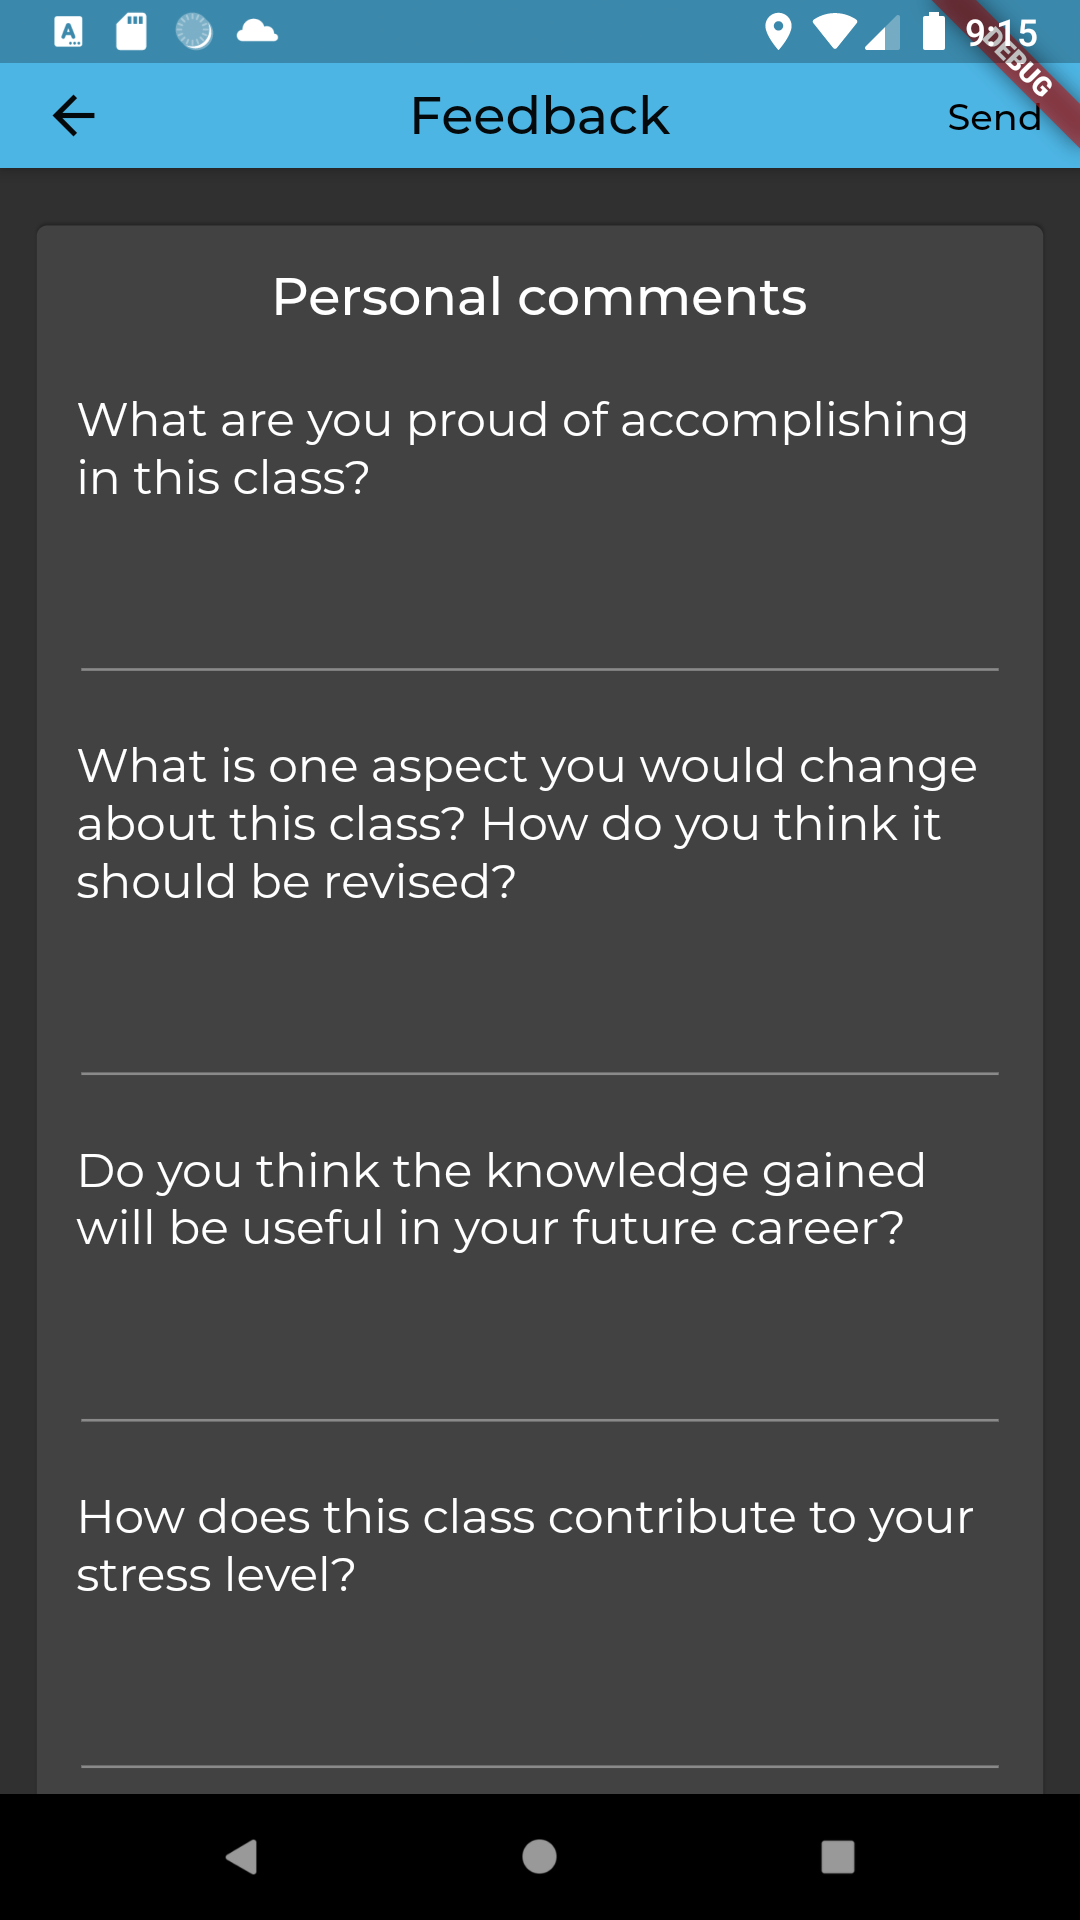
\includegraphics[width=0.3\textwidth]{figures/app/final/feedback_form_3.png}
            \caption{Feedback questionnaire page}
            \label{4:fig:feedback_form_page}
        \end{minipage}
    \end{figure}
    
    a specific form directly through this page by tapping an unchecked entry.
    
    \begin{figure}[!ht]
        \centering
        \begin{minipage}[t]{0.32\textwidth}
            \captionsetup{justification=centering}
            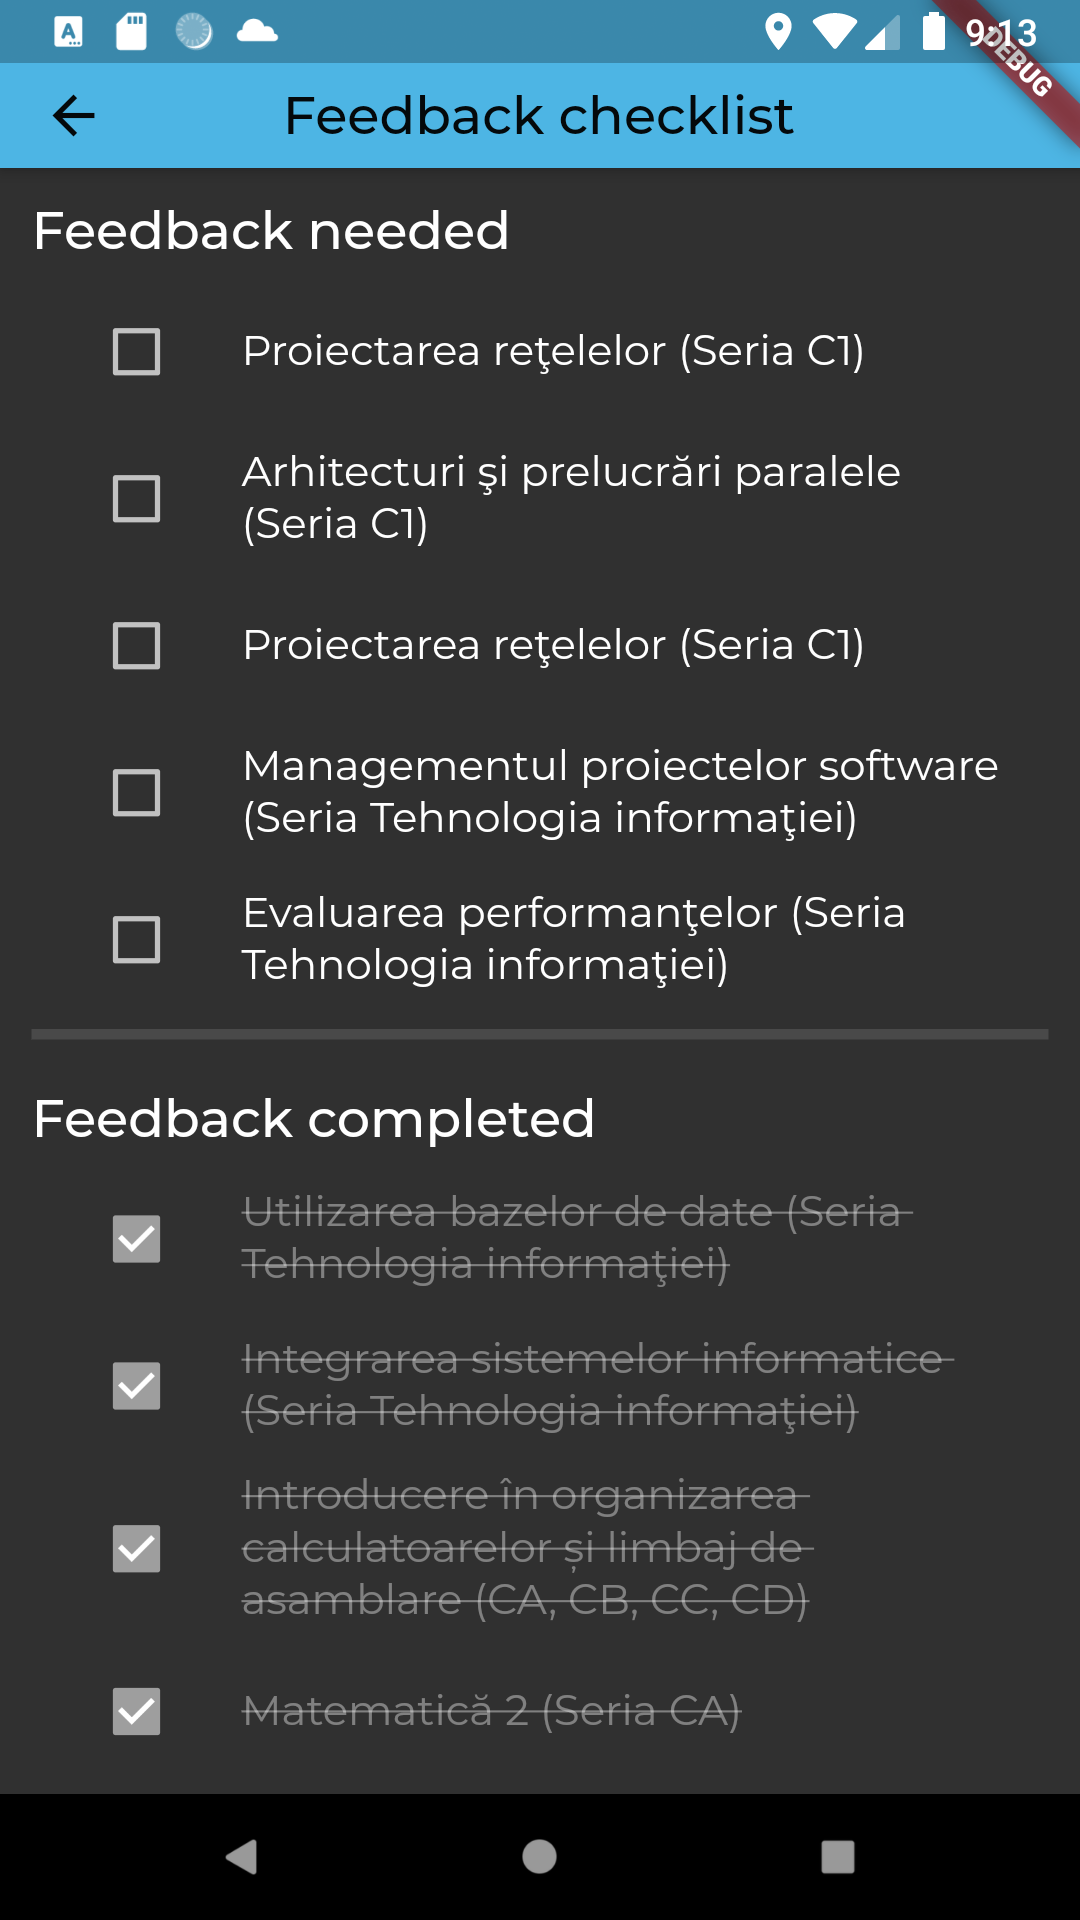
\includegraphics[width=\textwidth]{figures/app/final/feedback_checklist.png}
            \caption{Feedback checklist page}
            \label{4:fig:feedback_checklist}
        \end{minipage}
        \hfill
        \begin{minipage}[t]{0.663\textwidth}
            \captionsetup{justification=centering}
            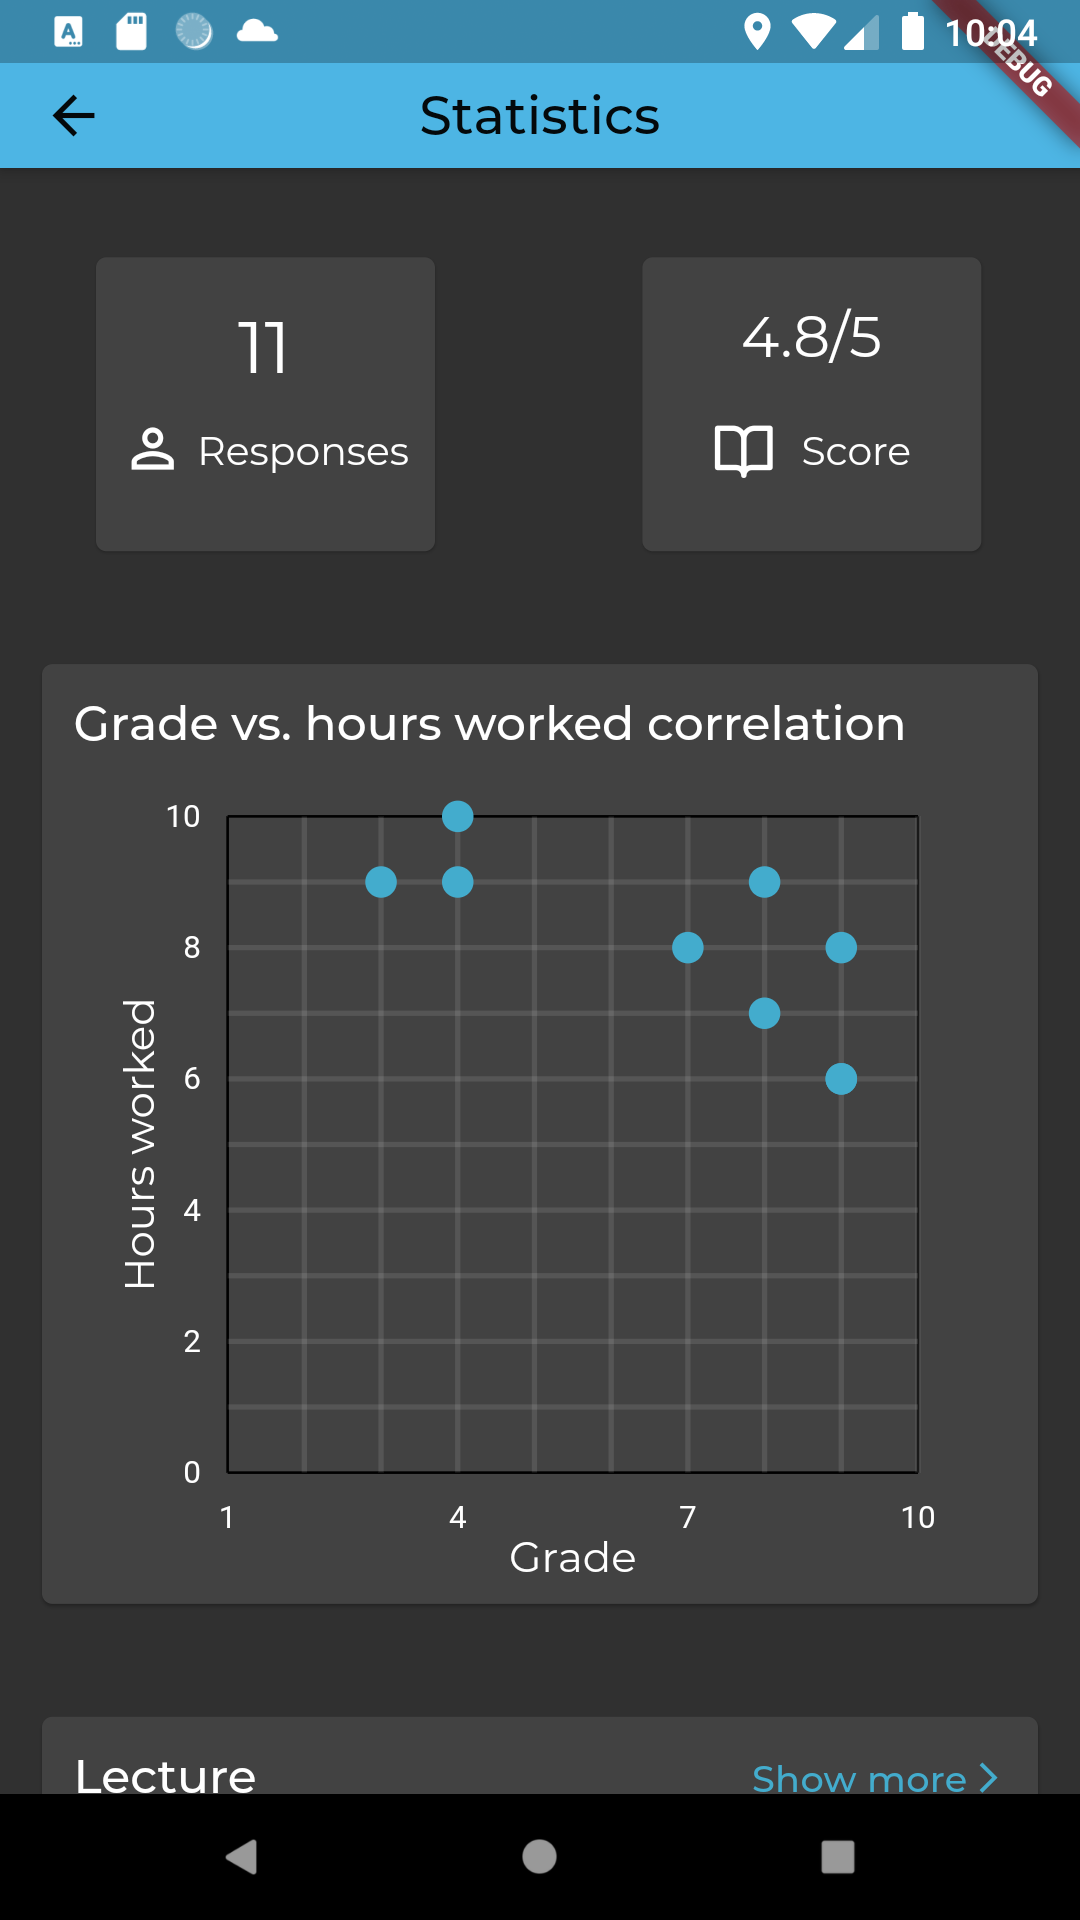
\includegraphics[width=0.485\textwidth]{figures/app/final/feedback_statistics_1.png}
            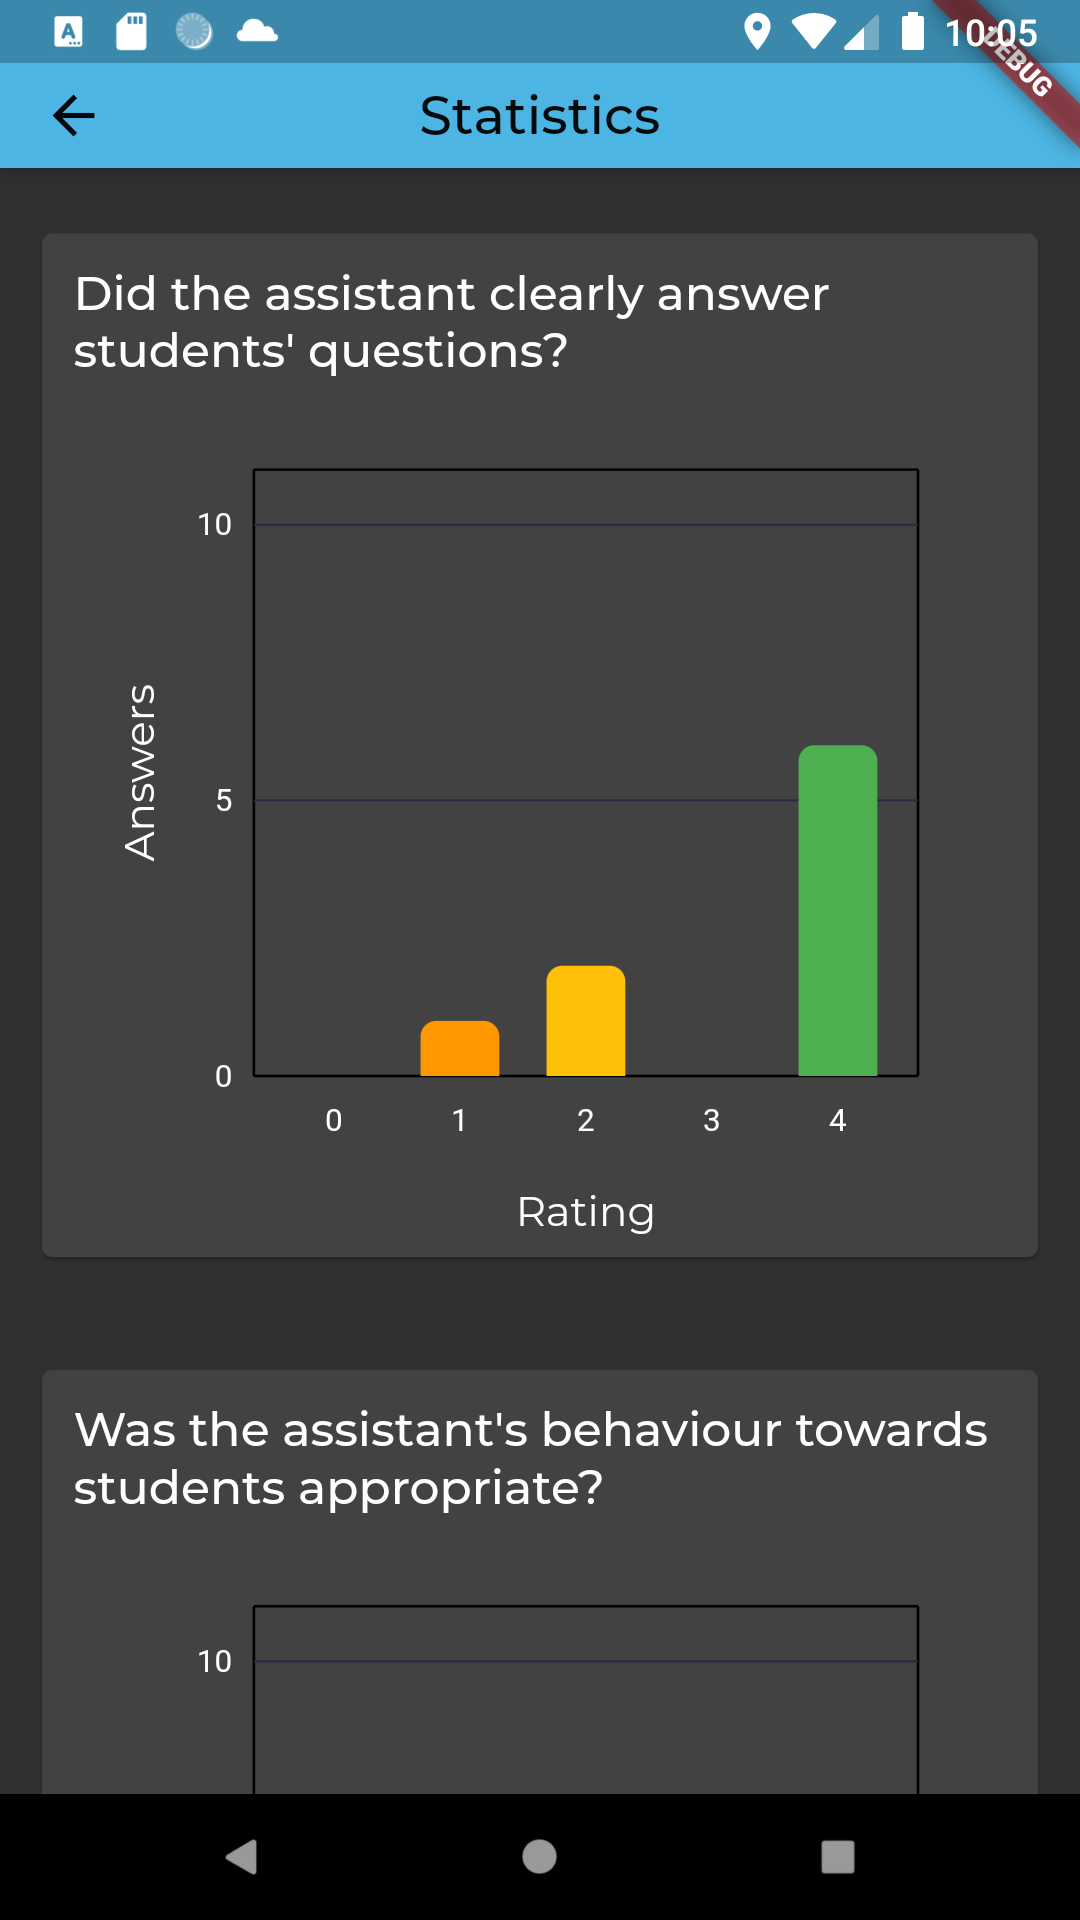
\includegraphics[width=0.485\textwidth]{figures/app/final/feedback_statistics_2.png}
            \caption{Feedback statistics page}
            \label{4:fig:feedback_statistics}
        \end{minipage}
    \end{figure}
    
    Our application offers students the opportunity to view statistics (fig. \ref{4:fig:feedback_statistics}) for each of their classes. Therefore, we emphasize the total number of students who shared their opinions and display a score computed as the arithmetic mean of all the ratings provided by students for each category of questions. Moreover, we added a scatter plot highlighting the correlation between the final grade and the average number of hours allocated to the study per week. To present the rest of the information collected from students, we have also introduced different bar charts or pie charts.
    
    The people page (fig. \ref{4:fig:people_page}) has a concise but straightforward and easy-to-use design. The search bar option (fig. \ref{4:fig:people_search}) is case-insensitive, and it is shown on the screen only after pressing the corresponding icon.
    